%%%%%%%%%%%%%%%%%%%%%%%%%%%%%%%%%%%%%%%%%%%%%%%%%%%%%%%%%%%%%%%%%%%%%%%%%%%%%%%%
%%%%%%%%%%%%%%%%%%%%%%%%%%%%%%%%%%%%%%%%%%%%%%%%%%%%%%%%%%%%%%%%%%%%%%%%%%%%%%%%
\exercice{Critère de Nyquist~\difficile}
%%%%%%%%%%%%%%%%%%%%%%%%%%%%%%%%%%%%%%%%%%%%%%%%%%%%%%%%%%%%%%%%%%%%%%%%%%%%%%%%
%%%%%%%%%%%%%%%%%%%%%%%%%%%%%%%%%%%%%%%%%%%%%%%%%%%%%%%%%%%%%%%%%%%%%%%%%%%%%%%%

Un système en boucle ouverte présente deux pôles instables (à parties réelles 
positives). On cherche à montrer que ce système peut être stable en 
modifiant la valeur du gain $K$ en boucle ouverte. La figure ci-dessous 
représente la réponse harmonique du système en boucle ouverte que l'on souhaite
asservir à l'aide d'une boucle de contre-réaction pour $K=-1$.
%-------------------------------------------------------------------------------
\begin{center}
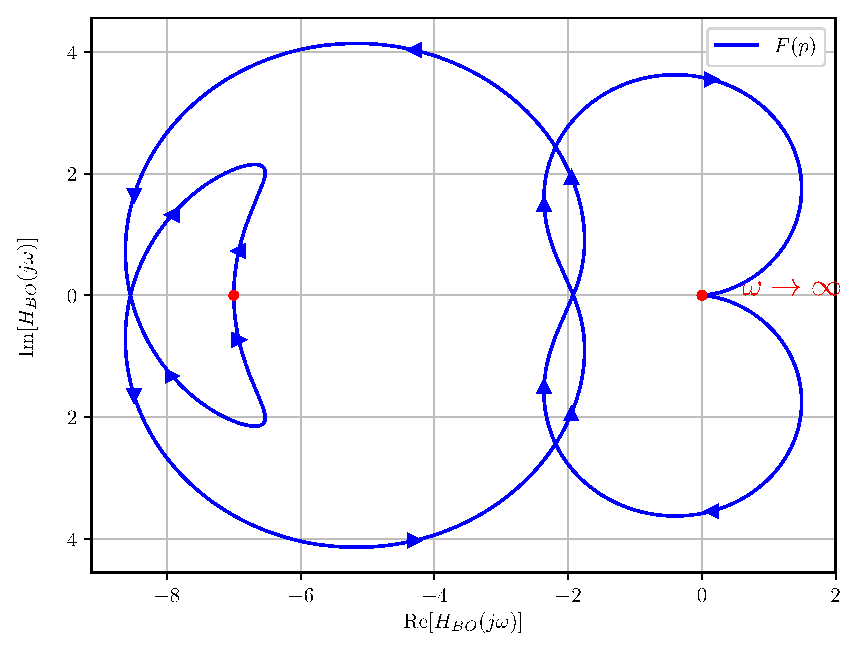
\includegraphics[width=0.8\textwidth]
                {fig/exercice_nyquist_chap_stab_ex1_enonce.eps}
\end{center}
%-------------------------------------------------------------------------------

%%%%%%%%%%%%%%%%%%%%%%%%%%%%%%%%%%%%%%%%%%%%%%%%%%%%%%%%%%%%%%%%%%%%%%%%%%%%%%%%
\question{D'après le critère de Nyquist, déterminer les zones du plan complexe 
qui permettraient au système d'être stable en boucle fermée.}
%%%%%%%%%%%%%%%%%%%%%%%%%%%%%%%%%%%%%%%%%%%%%%%%%%%%%%%%%%%%%%%%%%%%%%%%%%%%%%%%

%%%%%%%%%%%%%%%%%%%%%%%%%%%%%%%%%%%%%%%%%%%%%%%%%%%%%%%%%%%%%%%%%%%%%%%%%%%%%%%%
\question{Déterminer alors la condition sur $K$ pour ce système soit stable en 
boucle fermée.} 
%%%%%%%%%%%%%%%%%%%%%%%%%%%%%%%%%%%%%%%%%%%%%%%%%%%%%%%%%%%%%%%%%%%%%%%%%%%%%%%%

